\documentclass[tikz]{standalone}

% Import tikz
\usepackage{tikz}

\begin{document}

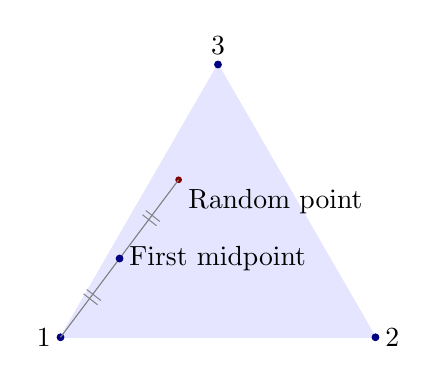
\begin{tikzpicture}
\coordinate (A) at (0,0); 
\coordinate (B) at (4,0); 
\coordinate (C) at (2,3.464);
\draw[fill, blue!10!white] (A) -- (B) -- (C) -- (A);
\draw[fill, blue!50!black] (A) circle (1.2pt) node[black,  left]{$1$};
\draw[fill, blue!50!black] (B) circle (1.2pt) node[black, right]{$2$};
\draw[fill, blue!50!black] (C) circle (1.2pt) node[black, above]{$3$};
\draw[fill, red!50!black] (1.5,2) circle (1pt)  node[black, below right]{Random point};
\draw[gray] (1.5,2) -- (0.75,1) node[gray,midway,rotate=-38,xshift=0.5pt]{=};
\draw[gray] (0.75,1) -- (A)     node[gray,midway,rotate=-38,xshift=0.5pt]{=};
\draw[fill, blue!50!black] (0.75,1) circle (1.2pt) node[black, right]{First midpoint};
\end{tikzpicture}

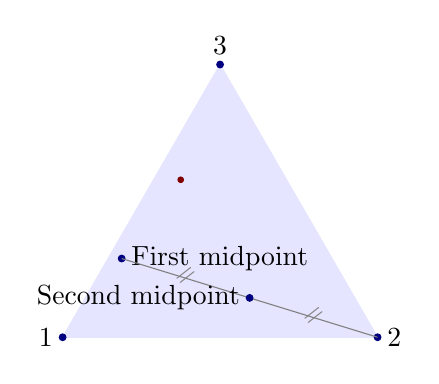
\begin{tikzpicture}
\coordinate (A) at (0,0); 
\coordinate (B) at (4,0); 
\coordinate (C) at (2,3.464);
\draw[fill, blue!10!white] (A) -- (B) -- (C) -- (A);
\draw[fill, blue!50!black] (A) circle (1.2pt) node[black,  left]{$1$};
\draw[fill, blue!50!black] (B) circle (1.2pt) node[black, right]{$2$};
\draw[fill, blue!50!black] (C) circle (1.2pt) node[black, above]{$3$};
\draw[fill, red!50!black] (1.5,2) circle (1pt)  node[black, below right]{};
\draw[fill, blue!50!black] (0.75,1) circle (1.2pt) node[black, right]{First midpoint};
\draw[gray] (0.75,1) -- (2.375,0.5) node[gray,midway,rotate=38,xshift=0.5pt]{=};
\draw[gray] (2.375,0.5) -- (B)      node[gray,midway,rotate=38,xshift=0.5pt]{=};
\draw[fill, blue!50!black] (2.375,0.5) circle (1.2pt) node[black, left]{Second midpoint};
\end{tikzpicture}

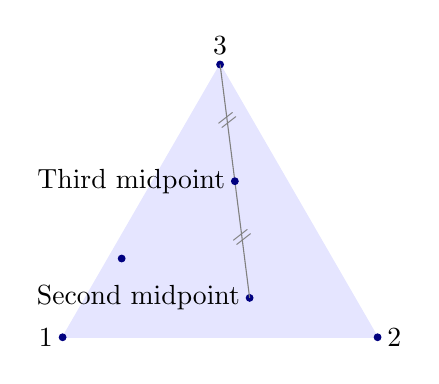
\begin{tikzpicture}
\coordinate (A) at (0,0); 
\coordinate (B) at (4,0); 
\coordinate (C) at (2,3.464);
\draw[fill, blue!10!white] (A) -- (B) -- (C) -- (A);
\draw[fill, blue!50!black] (A) circle (1.2pt) node[black,  left]{$1$};
\draw[fill, blue!50!black] (B) circle (1.2pt) node[black, right]{$2$};
\draw[fill, blue!50!black] (C) circle (1.2pt) node[black, above]{$3$};
\draw[fill, blue!50!black] (0.75,1) circle (1.2pt) node[black, right]{};
\draw[fill, blue!50!black] (2.375,0.5) circle (1.2pt) node[black, left]{Second midpoint};
\draw[gray] (2.375,0.5) -- (2.1875,1.982) node[gray,midway,rotate=38,xshift=0.5pt]{=};
\draw[gray] (2.1875,1.982) -- (C)         node[gray,midway,rotate=38,xshift=0.5pt]{=};
\draw[fill, blue!50!black] (2.1875,1.982) circle (1.2pt) node[black, left]{Third midpoint};
\end{tikzpicture}

\end{document}
